\documentclass{article} % For LaTeX2e
\usepackage{nips12submit_e,times}
\usepackage{amsmath,amsthm,amssymb, dsfont}
\usepackage{pgf, tikz}
\def\I{\mathbb{I}}
\def\R{\mathbb{R}}
\usetikzlibrary{arrows,automata}

\title{Modeling Infectious Knowledge in Collaborative Communities}


\author{
Eliana Feasley\\
Department of Computer Science\\
University of Texas at Austin\\
\texttt{elie@cs.utexas.edu} \\
\And
Wesley Tansey\\
Department of Computer Science\\
University of Texas at Austin\\
\texttt{tansey@cs.utexas.edu} \\
}

\newcommand{\fix}{\marginpar{FIX}}
\newcommand{\new}{\marginpar{NEW}}
\def\c{\textbf{ Cite }}
\nipsfinalcopy

\begin{document}

\maketitle

\begin{abstract}
The way that information infects different spaces of ideas is a crucial topic with applications to basic graph theory, epidemiology, machine learning, and marketing. In this paper, we examine the dynamics of information spread across communities with overlapping networks in several real-world domains. Each of these collaborative communities is structured such that it is possible to track how ideas spread over time and to discover latent subcommunities. We present an approximate graph structure inference algorithm that captures the most influential connections between subsites in a collaborative community. Additionally, we provide an approach for leveraging graphical models to predict the spread of memes through a community over time. The techniques we develop provide a framework for a new class of social network analysis.
\end{abstract}

\section{Introduction}
\label{intro}
Social cascades capture the concept of new ideas, or \textit{memes}, spreading across influence networks and infecting subcultures. Cascade theory has applications to several areas, including epidemiology, graph theory, machine learning, and marketing. In this paper, we examine the dynamics of information-spread across sub-communities with overlapping networks in several real-world domains: the social news site \textit{reddit}; the Meme Tracker dataset \cite{memetracker}, a collection of blogs and mainstream media; the question-answer network \textit{StackExchange}; and the general interest forum \textit{Something Awful}. Our goal is to capture the flow of memes by learning a graphical model for each domain. In this paper, we present approaches for inferring both the structure and weights of such models. Additionally, we model meme infections as timeseries to predict future topics and discover the structure of latent communities.

The remainder of this paper is organized as follows. Section \ref{sec:background} presents an overview of previous work on cascades. Section \ref{sec:structure} presents our algorithm for approximate structure learning in collaborative communities. Section \ref{sec:prediction} details the results of using graphical models to predict social cascades. Finally, section \ref{sec:conclusions} discusses potential future work.

\section{Background}
\label{sec:background}
The rise of online social media in recent years has created numerous opportunities for social cascade researchers. In this section, we discuss some of the techniques developed for studying cascades in social media, compare their applicability to collaborative communities, and differentiate them from our own approach.

\subsection{Collaborative Communities}
A \textit{collaborative community}, in this paper, is defined as any site or network of sites which has a single overall userbase and multiple subsites. Each user in the community is subscribed to at least one subsite and can optionally choose to subscribe to as many of the subsites as they like. Examples of such communities may include social news sites, question-answer sites, and discussion forums. Note that traditional friendship-based social networks are not valid collaborative communities, as users must be given permission to \textit{friend} other users. Similarly, microblogging sites do not qualify, as users are not able to comment directly on another user's feed.

\subsection{Social Cascades}
Social cascades have been investigated across several kinds of social networks. In \cite{info_contag}, following and friendship relationships are observed in order to explore the effect of explicit network structure on information cascades. In such networks, popularity of stories peaks with an age of about one day, and then subsides. 

Open networks, where all information is accessible to all users at all times, are fundamentally different in their behavior than closed networks, where information is private and must be shared through an explicit user action. Closed email chain networks were analyzed in \cite{viral_dynamics} and showed a short lifetime for viral information. In contrast, open networks have shown \cite{flickr} rapid spreading to a large and diffuse user base.

Structureless approaches have also been explored. In Twitter\footnote{http://twitter.com}, \textit{``bursty''} keywords can be aligned with trends -- entire topics that are becoming more popular \cite{twitter_trend}. In collaborative communities, however, we are interested in both the rise of such topics and the path they travel through the network of subsites.

\subsection{Structure Learning}
Networks of influence have been inferred in a variety of contexts. Contagion networks have been used \cite{contagion} to model the spread of disease throughout a social network. In marketing, contagion networks have been leveraged to identify how products and ad campaigns virally reach critical mass (i.e., ``go viral'') \cite{marketing1, marketing2}. In a more general context, NetInf \cite{netinf} was developed to infer directed network structure from a list of meme ``infections'' in a given network. Similarly, \cite{measuresocial} infers graphs to visualize and better analyze flows in social networks. While all of these approaches are powerful techniques, none quite fit the requirements of collaborative community network inference. Specifically, none are able to filter a fully-connected, undirected graph down to only the most influential connections in a manner amenable to probabilistic graphical inference as an exponential family.

\section{Learning Structure}
\label{sec:structure}
In this section, we present our approach to learning the structure of influence graphs in collaborative communities. We first present an overview of the general problem, followed by our approach to learning structure. Finally, we validate our method on three real-world datasets: \textit{reddit}, \textit{StackExchange}, and \textit{Something Awful}.

\subsection{Challenges for Collaborative Communities}
Learning graphical model structure is a particularly difficult task for collaborative communities. Each subsite forms a node in the network, and memes can potentially spread between any two subsites that share at least one user. In friendship-based social networks, we typically expect the percentage of mutual friends to be relatively low and edges exist simply as binary friend-or-not connections, resulting in a very sparse adjacency matrix. However, in collaborative communities with thousands of participants, it is reasonable to expect that most subsites share users, resulting in a nearly-complete adjacency matrix. A naive approach would thus result in a fully connected graph, which is undesirable as it yields little insight and may make certain tasks intractable.

\subsection{Approximate Structure Learning Algorithm}
\label{algorithm}
As it is possible for a meme to spread between any two subsites, any structure learning algorithm that yields a less-than-fully-connected graph is learning an approximate structure. As noted previously, an approximate structure may be desirable for gaining insights and reducing computational requirements. We next present our approximate structure learning algorithm for collaborative communities.

We first begin by defining an \textit{adjency matrix} $\mathcal{A}$ over subsites $\mathcal{S}$, such that $\mathcal{A} \in \R^{|\mathcal{S}|\times|\mathcal{S}|}$. For each pair $(s,t) \in \mathcal{A}$ of subsites, we mine the percentage of \textit{active} users that overlap in both $s$ and $t$. We define a user as \textit{active} if they have posted at least once on both subsites\footnote{Note that mining inactive users would be infeasible since most collaborative communities do not reveal the subsites to which a user subscribes.}:

$$
a(u) = \begin{cases}1&u \in P_s\text{ and }u \in P_t\\0 &\text{otherwise}\end{cases}
$$

where $P_i$ is the set of posts in subsite $i$. This yields the adjacency matrix:

$$
\mathcal{A}[s,t] = \sum_{\forall u \in \mathcal{U}}\dfrac{a(u)}{min(|\mathcal{U}^s|,|\mathcal{U}^t|)}
$$

where $\mathcal{U}$ is the set of active users and $\mathcal{U}^i$ is the set of active users in subsite $i$.

Rather than focusing on binary co-occurrence edges, our algorithm assesses the strengths of user overlap between two subsites and removes edges that are below a user-specified threshold. We define the relative strength matrix, $\mathcal{A}^*$:

$$
\begin{array}{lll}
\mathcal{A}^*[s,t] &=& \alpha \dfrac{\mathcal{A}[s,t] - \mu(\mathcal{A})}{\sigma(\mathcal{A})}\\
\end{array}
$$

where $\mu$ and $\sigma$ are the mean and standard deviation, respectively, and $\alpha$ is a tuning parameter. Finally, we define the weighted edge matrix, $\mathcal{E}$:

$$
\begin{array}{lll}
\mathcal{E}[s,t] &=& \begin{cases}\mathcal{A}^*[s,t] & \text{if }\mathcal{A}^*[s,t] \geq \gamma \\0 &\text{otherwise}\end{cases}\\
\end{array}
$$

where $\gamma$ is the user-specified strength threshold.

The resulting graph, $\mathcal{G} = (\mathcal{S},\mathcal{E})$, captures the most likely sources of influence for each node. To predict meme spreads, one could then convert $\mathcal{G}$ to a dynamic graphical model, $\mathcal{G}^*$. To do this, we introduce a set of $n$ timesteps, $T = \{ t_0, t_1, \dots, t_n\}$, such that the state of the nodes at a given time $t_i$ is represented by $\mathcal{S}_i$. $\mathcal{G}^*$ captures the transition from $t_i \rightarrow t_{i+1}$ as follows:

$$
\begin{array}{lll}
\mathcal{S}^*_i &=& S_i \cup S_{i+1},\\
\mathcal{E}^*_i[s,t] &=& \begin{cases}1 & \text{if } s \in \mathcal{S}_i\text{, }t \in \mathcal{S}_{i+1} \text{, and } \mathcal{E}[s,t] > 0\\
                                      1 & \text{if } s \in \mathcal{S}_{i+1}\text{, }t \in \mathcal{S}_{i+1} \text{, and } \mathcal{E}[s,t] > 0\\
                                      0 & \text{otherwise}\end{cases},\\
\mathcal{G}^*_i &=& (\mathcal{S}^*_i,\mathcal{E}^*_i).\\
\end{array}
$$

Queries to our dynamic graph will always be performed with the nodes in $\mathcal{G}_i$ being observed, thus connecting them would not affect the MAP inference for nodes in $\mathcal{G}_{i+1}$. One important point is that while the weights inferred by our algorithm could represent final weights in a graphical model, it is not clear that doing so would produce an accurate probability distribution.

\subsection{Experiments}
To validate our approach, we mined active user adjacency matrices for three real-world collaborative communities: \textit{reddit}, \textit{StackExchange}, and \textit{SomethingAwful}. The results for each community are presented next.

\subsubsection{reddit}
\textit{reddit}\footnote{http://reddit.com} is a social news community where each subsite\footnote{reddit subsites are called subreddits.} represents a different news topic. By default, all users are subscribed to a generic set of subsites such as \textit{politics} and \textit{humor}. The high degree of overlap among these default subsites produces a low signal-to-noise ratio in the adjacency matrix. Consequently, we first removed all default subsites from our dataset. To conform to our time constraints and maximize the amount of insight we could draw, we then limited the remaining non-default subsites to the top 25. The graph generated by our structure learning algorithm is shown in Figure \ref{fig:reddit}.

Two interesting properties of the graph immediately stand out. First, the explicit-content subreddits, \textit{nsfw}, \textit{sex}, and \textit{gonewild}, are clustered together, indicating that memes on these subreddits are not likely to spread to the rest of the network and memes within the cluster will quickly infect the remaining nodes. Conversely, the marijuana-oriented subreddit, \textit{trees}, is a super-node that appears to exert influence on nearly every node and vice-versa. Intuitively, we may thus hypothesize that the users of \textit{trees} are very influential on reddit and would thus expect to see memes spread from and to \textit{trees} rapidly.

\begin{figure}[htb]
\centering
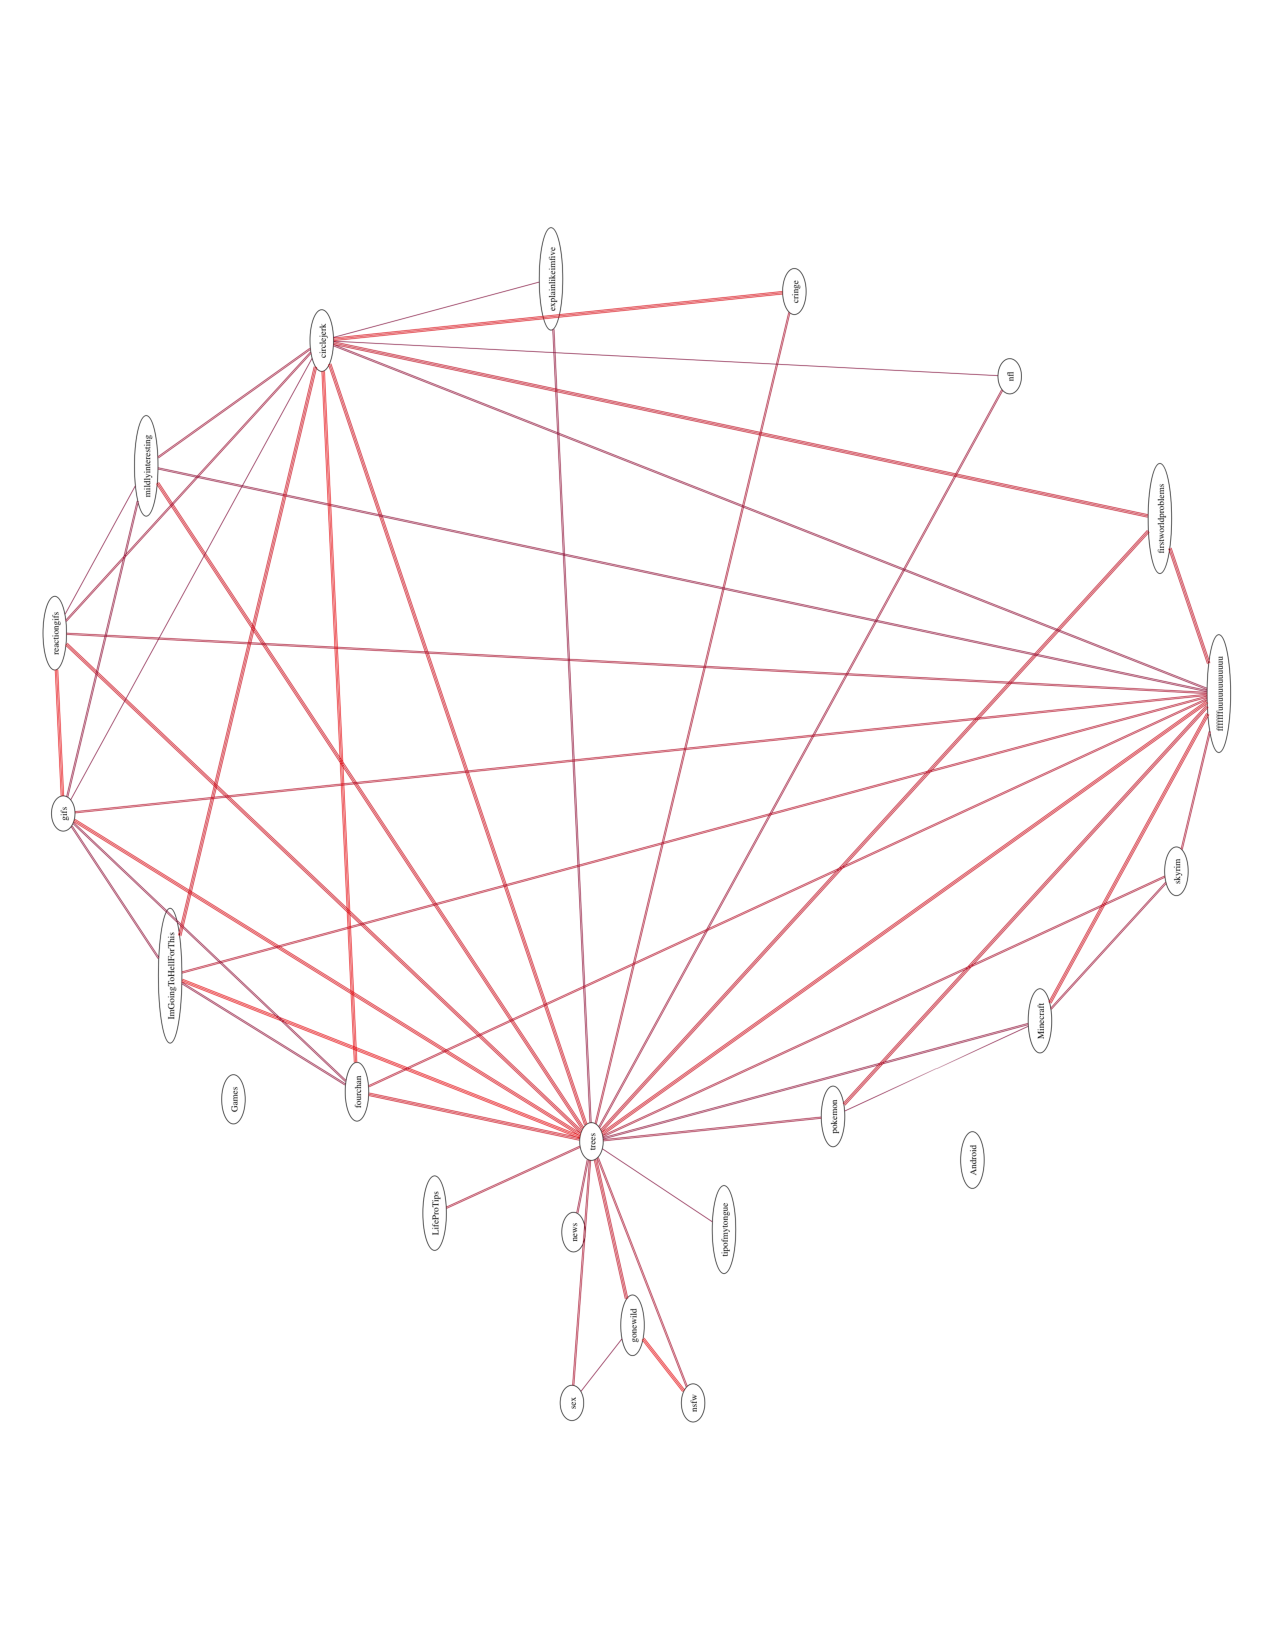
\includegraphics[width=\textwidth]{reddit.pdf}
\caption{Graph inferred from the top 25 non-default subreddits.}
\label{fig:reddit}
\end{figure}

\subsubsection{StackExchange}
\textit{StackExchange}\footnote{http://stackexchange.com} (SE) is a collaborative question-answer community where each subsite represents a different question topic. A majority of subsites focus on technical topics such as \textit{android} and \textit{security}, though non-technical subsites exist (e.g., \textit{cooking}). Memes in SE are likely to take the form of rising topics of interest, such as the popularity of iPhone games or Ruby on Rails. Unlike most collaborative communities, SE user subscription data is publicly available. We therefore used the adjacency matrix of all users to build our graph, shown in Figure \ref{fig:stackexchange}.

Perhaps counterintuitively, the \textit{stackoverflow} subsite has two orders of magnitude more overall users than other sites, but exerts no influence on the network. This may be a result of the other subsites being relatively unknown but having a strong sub-culture of shared users. Two high-influence pseudo-clusters appear between less technical and strictly technical sites in the upper-left and lower-right corners of the graph, respectively. Thus, localized memes may be frequent among these pseudo-clusters.

\begin{figure}[htb]
\centering
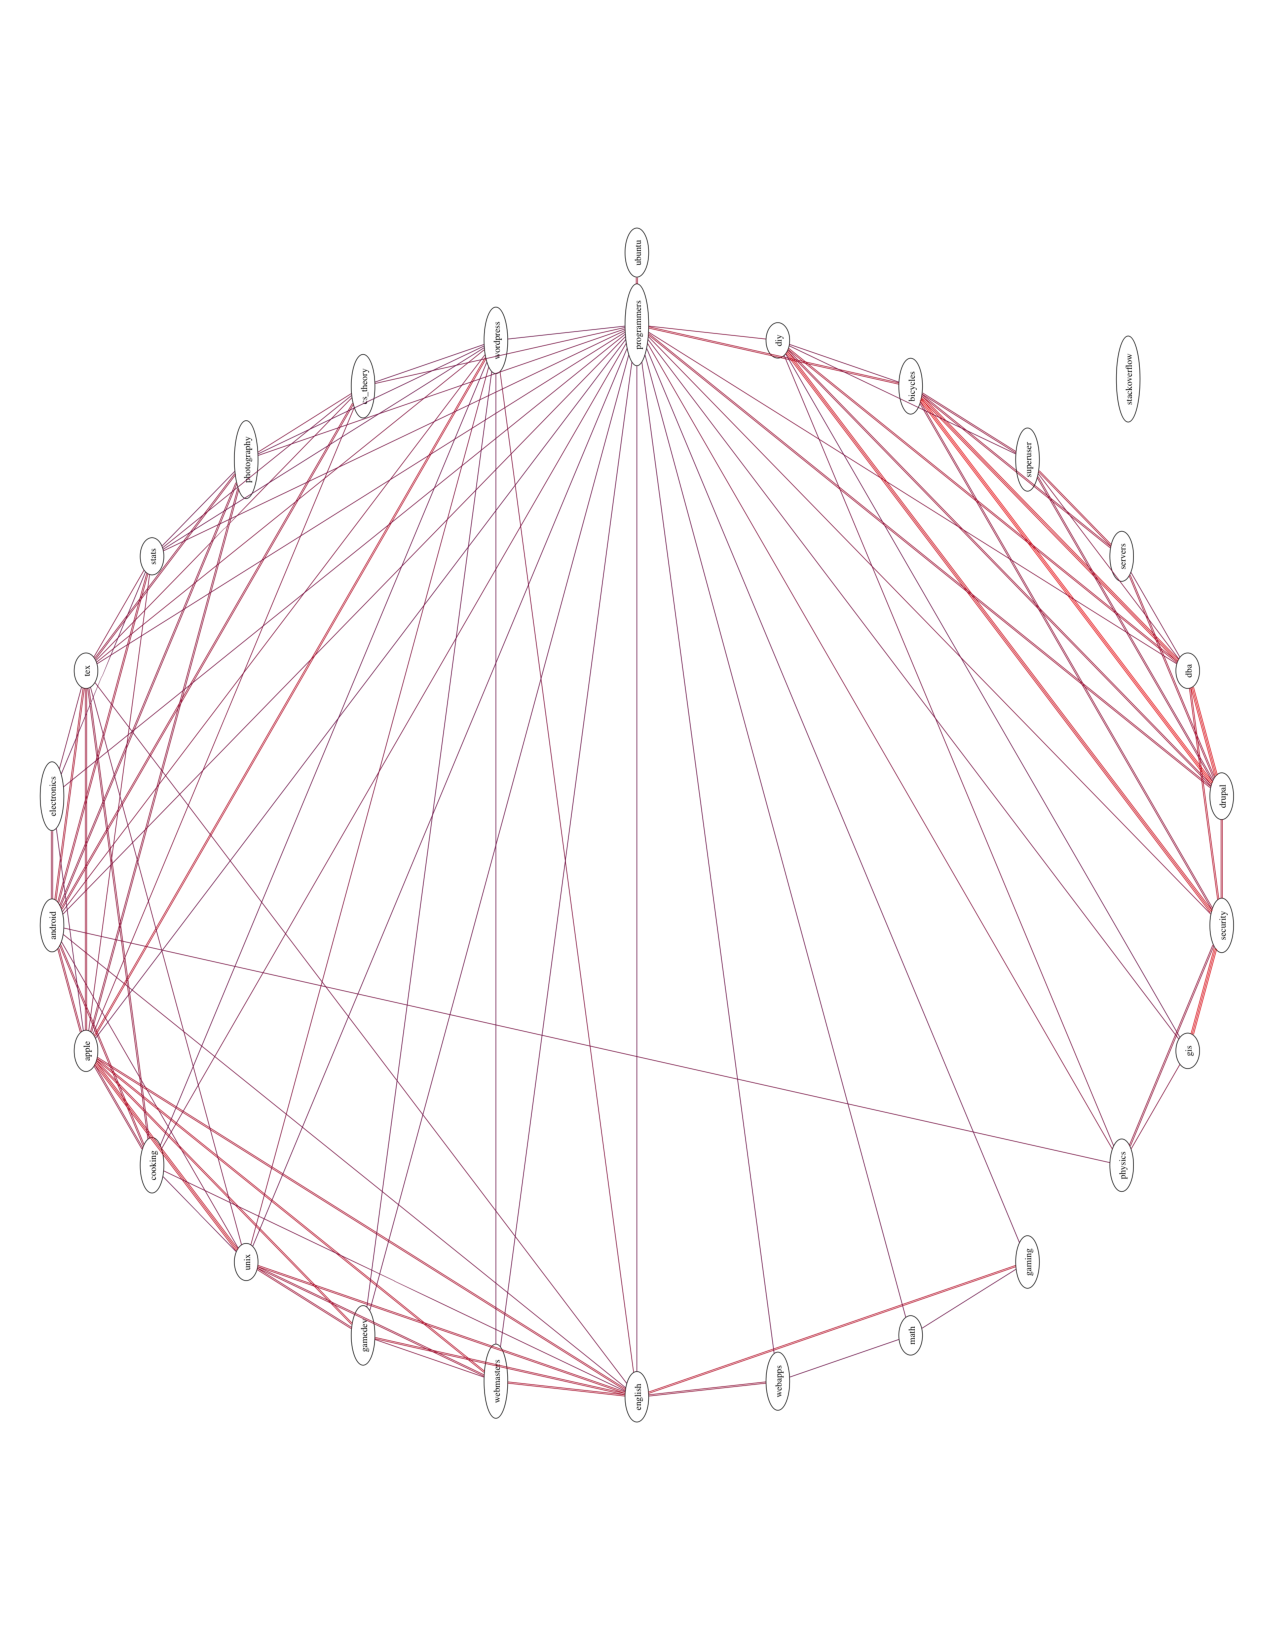
\includegraphics[width=\textwidth]{stackexchange.pdf}
\caption{Graph inferred from the 28 StackExchange subsites.}
\label{fig:stackexchange}
\end{figure}

\subsubsection{Something Awful}
\textit{Something Awful}\footnote{http://forums.somethingawful.com} (SA) is a general interest internet forum consisting of 53 subsites, where each subsite is a forum devoted to a separate topic such as games or books. SA is often regarded as a progenitor of memes, such as the infamous ``All your base are belong to us'' meme \cite{allyourbase}. The graph inferred from SA is shown in Figure \ref{fig:somethingawful}.

The SA graph reveals the important role of the main comedy subsite, \textit{Comedy Goldmine}. In contrast, the niche-specific subsites for music, football, and automobiles form clusters among their topics and exert virtually no influence on the broader site. Thus, intuitively, we would expect memes on Something Awful to originate from the comedy subsites and quickly spread to other general interest sites, but have little affect on niche subsites.

\begin{figure}[htb]
\centering
\includegraphics[width=\textwidth]{somethingawful.pdf}
\caption{Graph inferred from the 53 Something Awful subsites.}
\label{fig:somethingawful}
\end{figure}

\section{Predicting Cascades}
\label{sec:prediction}

Given a graph structure, we are faced with a difficult inference problem: detecting cascades in networks of subsites. We leverage the exponential family techniques from \cite{wainwright} to learn a parameterized model. In contrast to NetInf \cite{netinf}, where the strength of connections between sites is used merely to visualize and explore the data, we learn a probability distribution over nodes that can predict future data. We validate our approach on the Meme Tracker \cite{memetracker} dataset. Due to the time constraints of the project, we were unable to gather sufficient data from reddit, SE, or SA; these sites are left as future work.


\subsection{Problem statement}
Given a graphical model $\mathcal{G}^*_t = (\mathcal{S}^*_t, \mathcal{E}^*_t)$ created as specified in Section \ref{algorithm}, with nodes $s_{i,t} \in \mathcal{S}_t$ taking values 
$$
s_{i,t}=\begin{cases} 1 & $ if node $i$ is infected at time $t\\
                      0 & $otherwise$\end{cases} 
$$
 we want to predict the state of $\mathcal{S}_{t+1}$. Following the model in \cite{influential}, we refer to a node $s$ as becoming \textit{infected} with a given phrase if that phrase trended in $s$ during the last timestep. Once a node is infected, it is considered \textit{contagious.}

We model this domain as an unfolding Markov chain, where at each timestep nodes may become infected. Once infected with a meme, a node stays infected for the remainder of the time series. Figure \ref{fig:diagram} shows an example of this structure in which nodes $\{A,B,C\}$ represent the states of three subsites at time $t$, and nodes $\{A',B',C'\}$ represent the same subsites at time $t+1$.

\begin{figure}[htb]
\label{fig:diagram}
\centering
$$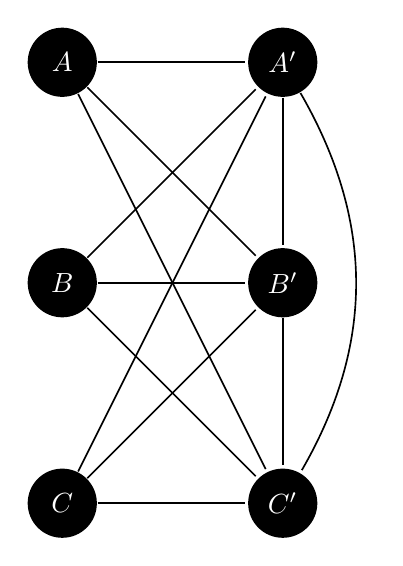
\begin{tikzpicture}[-,>=stealth',shorten >=1pt,auto,node distance=2.8cm,
                    semithick]
  \tikzstyle{every state}=[fill=black,draw=none,text=white]

  \node[state] (A)                    {$A$};
  \node[state]         (B) [below of=A] {$B$};
  \node[state]         (C) [below of=B] {$C$};
  \node[state]         (A1) [right  of=A] {$A'$};
  \node[state]         (B1) [right of=B] {$B'$};
  \node[state]         (C1) [right of=C] {$C'$};


  \path (A) edge        node {} (A1)
        (A) edge        node {} (B1)
        (A) edge        node {} (C1)
        (B) edge        node {} (A1)
        (B) edge        node {} (B1)
        (B) edge        node {} (C1)
        (C) edge        node {} (A1)
        (C) edge        node {} (B1)
        (C) edge        node {} (C1)
        (A1) edge        node {} (B1)
        (A1) edge [bend left] node {} (C1)
        (B1) edge        node {} (C1);
\end{tikzpicture}
$$
\caption{An example collaborative community network of three subsites.}
\end{figure}


\subsection{Learning Parameters}


We used the method for finding the MLE estimate in triangulated graphs described in \cite{wainwright} to learn the weights of our edges. The model is trained on every example graph $\mathcal{G}^*_t$ in the dataset. We define indicator functions 
$$\I_{s;j}=\begin{cases}1&$Node $s$ is in state $j\\0& s $ is not uninfected$\end{cases}, \forall s\in \mathcal{S}^*_t$$ 
and
$$\I_{r,s;j,k}=\begin{cases}1&$ Node $r$ is in state $j$  and node $s$ is in state $k\\
0& $otherwise$\end{cases},  \forall r,s\in \mathcal{E}^*_t.$$ 

Parameters $\hat{\theta}$ are the logs of the expectations of these indicator functions as defined in \cite{wainwright}.

We define the probability of an assignment to $\mathcal{S}_{t+1}$ given our graph $\mathcal{G}^*_t$ and $\mathcal{S}_t$  to be
  $$p_{\hat{\theta}}(\mathcal{S}_t^*)
  =\exp \left\{ \sum_{s\in \mathcal{S}}\hat{\theta}_s(\mathcal{S}_t^*)+\sum_{s,t\in \mathcal{E}}\hat{\theta}_{st}(\mathcal{E}_t^*)\right\} .$$


\subsection{Experiment and Results}

Our algorithm is evaluated on the Memetracker dataset used in \cite{memetracker}. Due to time constraints, we leave the evaluation of the three collaborative communities from Section \ref{sec:structure} as future work.

The Meme Tracker dataset is a collection of popular news sites scraped during the US presidential campaign season of 2008. Sites in the dataset are divided into two categories: blogs and major media sources. Memes detected via the Memetracker algorithm \cite{memetracker} are designated infections. This experiment uses the 20 most popular webssites and the 40 most popular blogs to evaluate the performance of our learning algorithm. We validated our approach by measuring the accuracy of our model using $4$-fold cross-validation, with a $~1\%$ holdout size per fold.

Accuracy in these experiments is denoted by the percentage of nodes correctly predicted by our algorithm for timestep $t+1$ given the nodes in timestep $t$. Our model relies on hill climbing to find a potential MAP assignment over nodes in $t+1$. The results of our experiment are shown in Table \ref{tab:results}.

\begin{table}
\centering
\begin{tabular}{|l|l|l|l|l|}
\hline
Fold & Total & Complete Matches & \% Matches & Avg. \% Nodes Correct   \\ \hline
0 & 8314 & 3130 & 0.3765 & 0.7512  \\ \hline
1 & 9216 & 3194 & 0.3466 & 0.7141  \\ \hline
2 & 7537 & 2937 & 0.3897 & 0.7910  \\ \hline
3 & 8036 & 3503 & 0.4360 & 0.7931 \\ \hline   
\end{tabular}
\caption{The results of our four-fold cross-validation on the Meme Tracker dataset.}
\label{tab:results}
\end{table}

\section{Discussion and Future Work}
\label{sec:conclusions}

One of the major difficulties of researching infections in social networks is the degree of sparsity. If a site is only infected when a meme is present, the graph is very sparse, and phenomena like a user absorbing content at time $t-1$ and then reproducing it on another site at time $t+1$ are difficut or impossible to model. However, if a site becomes infected with the first occurance of a meme and stays infected forever, information about when a meme is first flaring or when it hasn't been active in the last several timesteps is lost.

Important future work includes reformulating this problem with real values. In every formulation of the problem thus far, an infection is either present or not present. Real-valued indicators of the presence of an infection will help with the problem of information loss and sparsity.

Finally, time constraints on the project prohibited gathering sufficient data on the reddit, SE, and SA communities from Section \ref{sec:structure} to identify memes. We plan to continue scraping this data over the coming months and generate datasets comparable in size and scale to that of the Meme Tracker dataset.

\bibliography{sources}{}
\label{refs}
\bibliographystyle{plain}

\end{document}